% 02.06.2016 12:00 CET last changed by a.holzinger
% General Template for LNCS and LNAI contributions based on llncs, adapted by ah
% Many thanks to the TRS team
% In case of using eps compile via 1) TeXify and then proceed with 2) dvi2pdf
%
\documentclass{llncs}
\usepackage{float}

\usepackage[dvips]{graphicx}
\usepackage[ruled,vlined]{algorithm2e}
\usepackage{amsfonts}
\usepackage{amssymb}
\usepackage{amsmath}
\usepackage{mathtools}

\providecommand{\abs}[1]{\lvert#1\rvert}
\providecommand{\norm}[1]{\lVert#1\rVert}

\usepackage{calc}
\usepackage{subfigure}

\usepackage{color}
\usepackage{soul}
\usepackage{comment}

\newtheorem{prop}{Property}

\newenvironment{Bitemize}{\renewcommand\labelitemi{\textbullet}\begin{itemize}}{\end{itemize}}

\begin{document}

\title{The right to be forgotten:\\
Towards interactive Machine Learning on perturbed knowledge bases}

\author{Bernd Malle, Peter Kieseberg, Edgar Weippl, Andreas Holzinger}
\institute{Holzinger Group HCI-KDD \\
Institute for Medical Informatics, Statistics \& Documentation\\
            Medical University Graz, Austria\\
            \texttt{b.malle@hci-kdd.org}}

\maketitle

\begin{abstract}
	
The amount of patient-related data produced in today’s clinical setting poses many challenges with respect to collection, storage and responsible use. For example, in research and public health care analysis, data must be anonymized before transfer, for which the k-anonymity measure was introduced and successively enhanced by further criteria. As k-anonymity is an NP-hard problem, modern approaches often make use of heuristics based methods. This paper will convey the motivation for anonymization followed by an outline of its criteria as well as a general overview of methods \& algorithmic approaches to tackle the problem. As the resulting data set will represent a trade-off between utility and individual privacy, we need to optimize those measures to individual (subjective) standards. Moreover, the efficacy of an algorithm strongly depends on the background knowledge of a potential attacker as well as the underlying problem domain. Therefore, it seems logical to adapt the process including expert domain knowledge, which can be done via an interactive machine learning (iML) approach. We will therefore point out how domain experts might get involved to improve upon current methods and introduce an example setup based on the SaNGreeA algorithm; due to this algorithm's nature of taking into account structural (network) as well as information properties of the underlying problem domain, it can be useful for (but also limited to) common tabular data anonymization. Finally, we present our work by demonstrating a Web-based User Interface to conduct interactive machine learning tasks and compare the results of a variety of different parameter settings from our iML experiments with a standard industry anonymization algorithm in terms of efficiency, information loss as well as threat scenarios.

\medskip

\textbf{Keywords}: machine learning, interactive machine learning, anonymization, k-anonymity, SaNGreeA, information loss, structural loss, cost weighing vector


\end{abstract}

\renewcommand{\thesubfigure}{\thefigure.\arabic{subfigure}}
\makeatletter
\renewcommand{\p@subfigure}{}
\renewcommand{\@thesubfigure}{\thesubfigure:\hskip\subfiglabelskip}
\makeatother

\section{Introduction and Motivation for Research}

Privacy preserving machine learning \cite{DuchiJordan:2014:PrivacyAwareLearning} is an issue of increasing importance, fostered by anonymization \cite{Samarati:2001:kAnonymity}, in which a record is released only if it is indistinguishable from $k$ other entities in the data. However, k-anonymity is highly dependent on spatial locality in order to effectively implement the technique in a statistically robust way, and in arbitrarily high dimensions data becomes sparse, hence, the concept of spatial locality is not easy to define. Consequently, it becomes difficult to anonymize the data without an unacceptably high amount of information loss \cite{Aggarwal:2005:kAnonymity}. Therefore the problem of k-anonymization is on the one hand NP-hard, on the other hand the quality of the result obtained can be measured at the given factors: \emph{k-anonymity} means that attributes are suppressed or generalized until each row in a database is identical with at least $k-1$ other rows \cite{Sweeney:2002:k-Anonymity}; \emph{l-diversity} as extension of the k-anonymity model reduces the granularity of data representation by generalization and suppression so that any given record maps onto at least $k$ other records in the data \cite{MachanavajjhalaEtAl:2007:l-Diversity}; \emph{t-closeness} is a refinement of l-diversity by reducing the granularity of a data representation, and treating the values of an attribute distinctly by taking into account the distribution of data values for that attribute \cite{LiEtAl:2007:t-closeness}; and \emph{delta-presence}, which links the quality of anonymization to the risk posed by inadequate anonymization \cite{NergizClifton:2010:Delta-Presence}, but not with regard to the actual security of the data, i.e., the re-identification through an attacker. For this purpose, certain assumptions about the background knowledge of the hypothetical enemy must be made. With regard to the particular demographic and cultural clinical environment this is best done by a human agent. Thus, the problem of (k-)anonymization represents a natural application domain for interactive Machine Learning (iML) with an human-in-the-loop \cite{Holzinger:2016:iML}, \cite{Kieseberg:2016:Doctor-in-the-Loop},  \cite{iMLExperiment}.

\begin {comment}
\section{Glossary and Key Terms}
NOTE: this section may not to be used for a conference
\textbf{Note: This is only for use when producing a Springer LNCS SOTA State-of-the-Art-Analysis paper}
\\[0,2cm]
\emph{SaNGreeA} is the abbreviation for Social Network Greedy Anonymization, which describes an anonymization algorithm which takes into account information loss as well as structural loss (from anonymizing the neighborhood of a network node). It is said to be greedy as it uses greedy clustering under the hood in order to avoid having to sift through an exponential solution space to find an optimum.

\end{comment}

\section{Basic Concepts}
\label{sect:basic_concepts}

\subsection{Tabular anonymization}
\label{ssect:tab_anonym}

Taking a look at Figure~\ref{fig:anon_categories} will help the reader in understanding the original (tabular) concept of anonymization: Given an input table with several columns, we will probably encounter three different categories of data:

\begin{itemize}
	\item \textbf{Personal identifiers} are data items which directly identify a person without having to cross-reference or further analyze them. Examples are first and last names, but even more so an (email) address or social security number (SSN). As personal identifiers are dangerous and cannot be generalized (see Figure~\ref{fig:gen_hierarchy}) in a meaningful way (e.g. one could generalize the \textit{address} field, which would only result in some kind of Zip code), this category of data is usually removed. The table shows this column in a red background color.
	\item \textbf{Sensitive data,} also called 'payload', which is the kind of data we want to convey for statistics or research purposes. Examples for this category would be disease classification, drug intake or personal income level. This data shall be preserved in the anonymized dataset and can therefore not be deleted or generalized. The table shows this column in a green background color.
	\item \textbf{Quasi identifiers}, colored in the table with an orange background, are data that in themselves do not directly reveal the identity of a person, but might be used in aggregate to reconstruct it. For instance, \cite{sweeney2002k} mentioned that 87\% of U.S. citizens in 2002 had reported characteristics that made them vulnerable to identification based on just the 3 attributes \textit{zip code}, \textit{gender} and \textit{date of birth}. But although this data can be harmful in that respect, it might also hold vital information for the purpose of research (e.g. zip code could be of high value in a study on disease spread). The solution - and this is the actual point of all anonymization efforts - is to generalize this kind of information, which means to lower its level of granularity. As an example, one could generalize the ZIP codes 41074, 41075 and 41099 to a generalized version 410**, as shown in Figure~\ref{fig:anonymized_clusters}.
\end{itemize}

\begin{figure}[!t]
	\begin{center}
		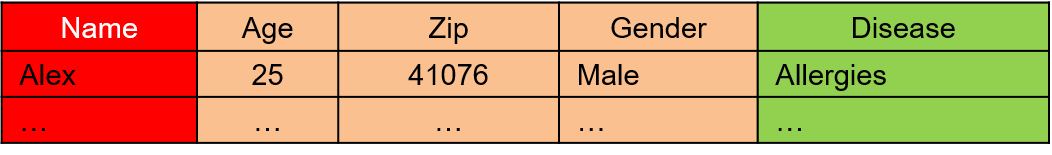
\includegraphics[width=0.9\textwidth]{figures/anonym/3typesofdata}
		\caption{The three types of data considered in (k-)anonymization}
		\label{fig:anon_categories}
	\end{center}
\end{figure}

As described in \cite{ciriani2007kappa}, k-anonymization requires that in each data release every combination of values of quasi-identifiers must be identical to at least $k-1$ other entries in that release, which can be seen as a clustering problem with each cluster's (in the context of anonymization also called an 'equivalence class') internal quasi-identifier state being identical for every data point. This can be achieved via suppression and generalization, where suppression means simply deletion, whereas in generalization we try to retain some usable value.

The process of generalization works through a concept called \textit{generalization hierarchies}, which form a tree, whose root denotes the most general value available for a data category (usually the 'all' value) and then branches to more and more specific occurrences, with its leafs representing the set of exact, original values (see Figure~\ref{fig:gen_hierarchy}). In generalizing some original input value, one traverses the tree from the leaf level upwards until a certain prerequisite is fulfilled. Usually, this prerequisite comes in the form of the k-anonymity requirement, so that we want to find a group of other data rows (=vectors) whose (generalized) quasi identifiers match the data point being processed.

\begin{figure}[!t]
	\begin{center}
		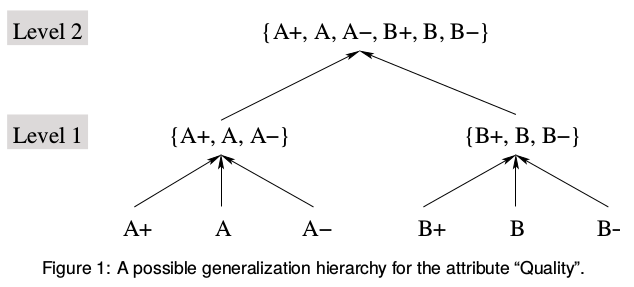
\includegraphics[width=0.8\textwidth]{figures/anonym/gen_hierarchy}
		\caption{Example of a typical generalization hierarchy}
		\label{fig:gen_hierarchy}
		\small
		taken from \cite{aggarwal2005approximation}
	\end{center}
\end{figure}


Each level of generalization involves a certain cost in information loss though, which means we do not just want to construct our clusters in any sequence possible, but minimize the overall information loss. This makes k-anonymization an NP-hard optimization problem (because of an exponential number of possible generalized quasi-identifier combinations), leaving us to conclude that the k-Anonymity problem is to lose as little information as possible in a dataset while ensuring that the release (the anonymized, publishable version of the dataset) satisfies the k-anonymization criterion \cite{aggarwal2005approximation}.

\begin{figure}[!t]
	\centering
	\begin{minipage}[b]{0.5\textwidth}
		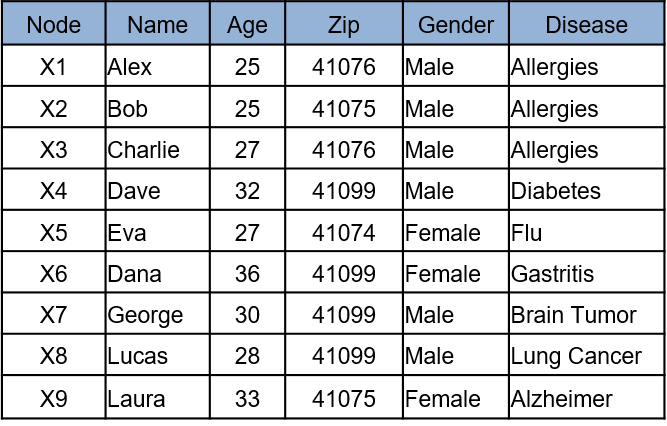
\includegraphics[width=\textwidth]{figures/anonym/k_anon_input}
	\end{minipage}
	\hfill
	\begin{minipage}[b]{0.418\textwidth}
		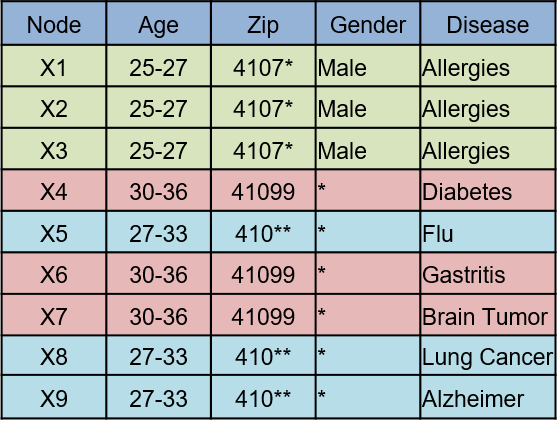
\includegraphics[width=\textwidth]{figures/anonym/k_anon_output}
	\end{minipage}
	\caption{Tabular anonymization: input table and anonymization result}
	\label{fig:anonymized_clusters}
\end{figure}


\subsection{Graph (social network) anonymization}
\label{ssect:graph_sn_anon}

In the last section we were solely concerned with tabular data; However, as social networks have gained huge popularity over the previous decade, and even modern medical databases come in the form of graph structures, the question of how to efficiently anonymize networks has gained ever more significance over the years.

As a start, one could see a graph just as a collection of nodes, where each node contains some kind of feature vector, akin to the row in a data table. Adopting that view, we could be tempted to simply ignore the existence of edges and apply some kind of algorithm suitable to the anonymization of tabular data. The main problem with this however lies in the fact that the structural environment of a node (the constellation of its neighbors within the greater network) provides some additional information. That is, even if we successfully (k-)anonymize the feature vectors of a graph according to the methods found in the previous chapter, we still run the risk of leaving to much information in the form of a known local subgraph structure.

Consider Figure~\ref{fig:anon_sn_problem} for example, in which the nodes of a graph have already been k-anonymized into groups of size 3 and 7, respectively. In this figure, local subgraphs b) and c) are actually (3)-anonymized, because as each node has the exact same local neighborhood structure, the additional information of a node possessing a degree of 0 (or 2) is of no additional value. For local subgraphs a) and d) on the other hand, the additional information of a node being of degree (x) has the potential to reveal its identity, as it is not indistinguishable from its neighbors within the equivalence class any more.

\begin{figure}[!t]
	\begin{center}
		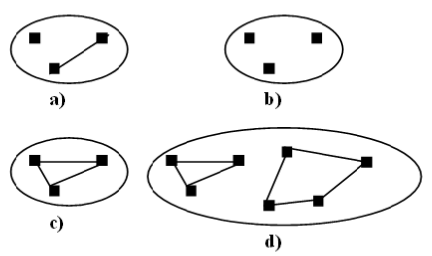
\includegraphics[width=0.8\textwidth]{figures/anonym/sn_problem}
		\caption{Local subgraph neighborhoods as additional anonymization obstacle.}
		\label{fig:anon_sn_problem}
	\end{center}
	\small
	(Example taken from \cite{campan2009data}.)
\end{figure}


\section{Related work}
\label{sect:related_work}


Several methods have been proposed to make re-identification of nodes in anonymized social graphs harder.	\cite{chester2011k} for example introduce the idea of vertex addition to labeled and unlabeled datasets. While an algorithm on the former remains NP complete, they provide an efficient ($O(nk)$) algorithm for unlabeled data. Experimenting on several well known datasets, they show that commonly-studied structural properties of the network, such as clustering coefficient, are only minorly distorted by their anonymization procedure.

Person re-identification is both a hard and important problem in many different domains and is challenging. Most approaches aim to model and extract distinctive and reliable features. However, seeking an optimal and robust similarity measure that quantifies a wide range of features against realistic conditions from a distance is still an open and unsolved problem for person reidentification  reidentification techniques \cite{Zheng:2013:reidentification}. 

In order to develop protection techniques in social networks it is necessary to consider three aspects \cite{Zhou:2008:SurveyAnonNetwork}: 1) the privacy information which may be
under attack; 2) the background knowledge that an adversary may use to attack the privacy
of target individuals; and 3) a specification of the usage of the published social network data so that an anonymization method can try to retain the utility of the data as much as possible whilst the privacy is preserved. 

The authors of \cite{kapron2011social} take the approach of adding edges to an edge-labeled graph like the Netflix movie database (with users and movies being nodes and edge weights representing movie ratings). They define tables as bipartite graphs and prove NP-hardness for the problems of neighborhood anonymity, i-hop anonymity and k-symmetry anonymity.

\cite{campan2009data}, whose local subgraph problem we already encountered, proposed a solution in the form of a greedy clustering algorithm which takes into account not only the information loss incurred by generalizing features of nodes, but also introducing a structural loss function based on the local neighborhood within an equivalence class (and between them). The author of this thesis implemented that approach utilizing GraphiniusJS and will demonstrate the algorithm in Section~\ref{sect:aoa_anonymization} as well as the anonymized results in Appendix Section~\ref{sect:anon_output_data}.


\section{Experiments}
\label{sect:experiments}


\subsection{Data} 
\label{ssect:data}


\begin{figure}[H]
	\begin{center}
    \hspace*{-1cm}
		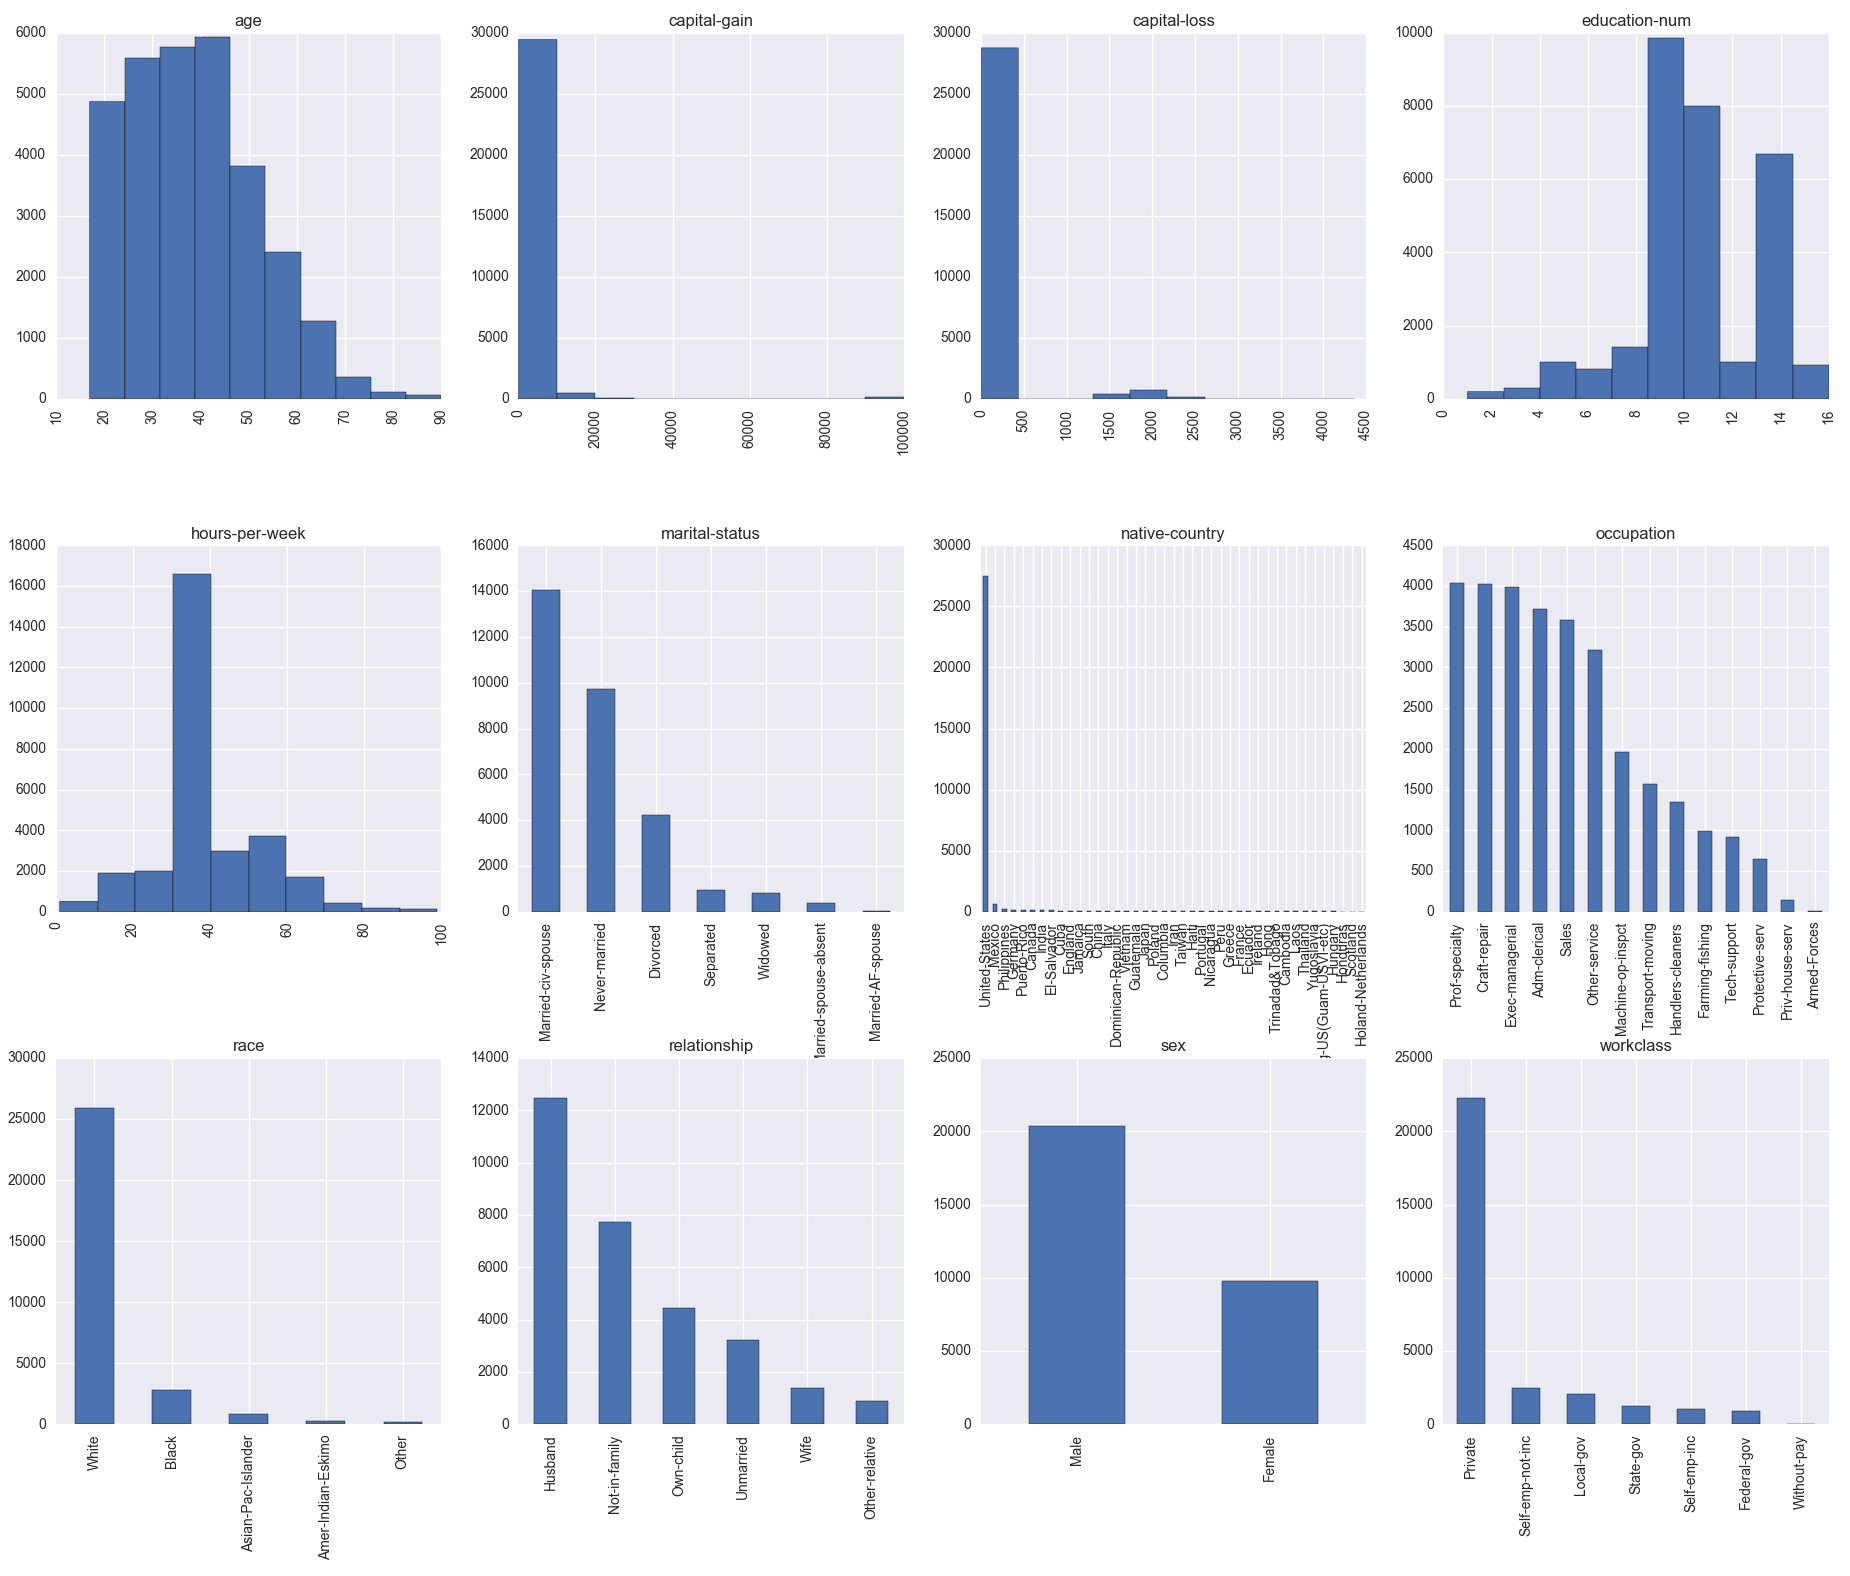
\includegraphics[width=1.2\textwidth]{figures/experiment/initial_distribution}
		\caption{Initial distribution of the data columns of the adult dataset}
		\label{fig:adult_original_distribution}
	\end{center}
\end{figure}

\begin{figure}[H]
	\begin{center}
    	\hspace*{-1cm}
		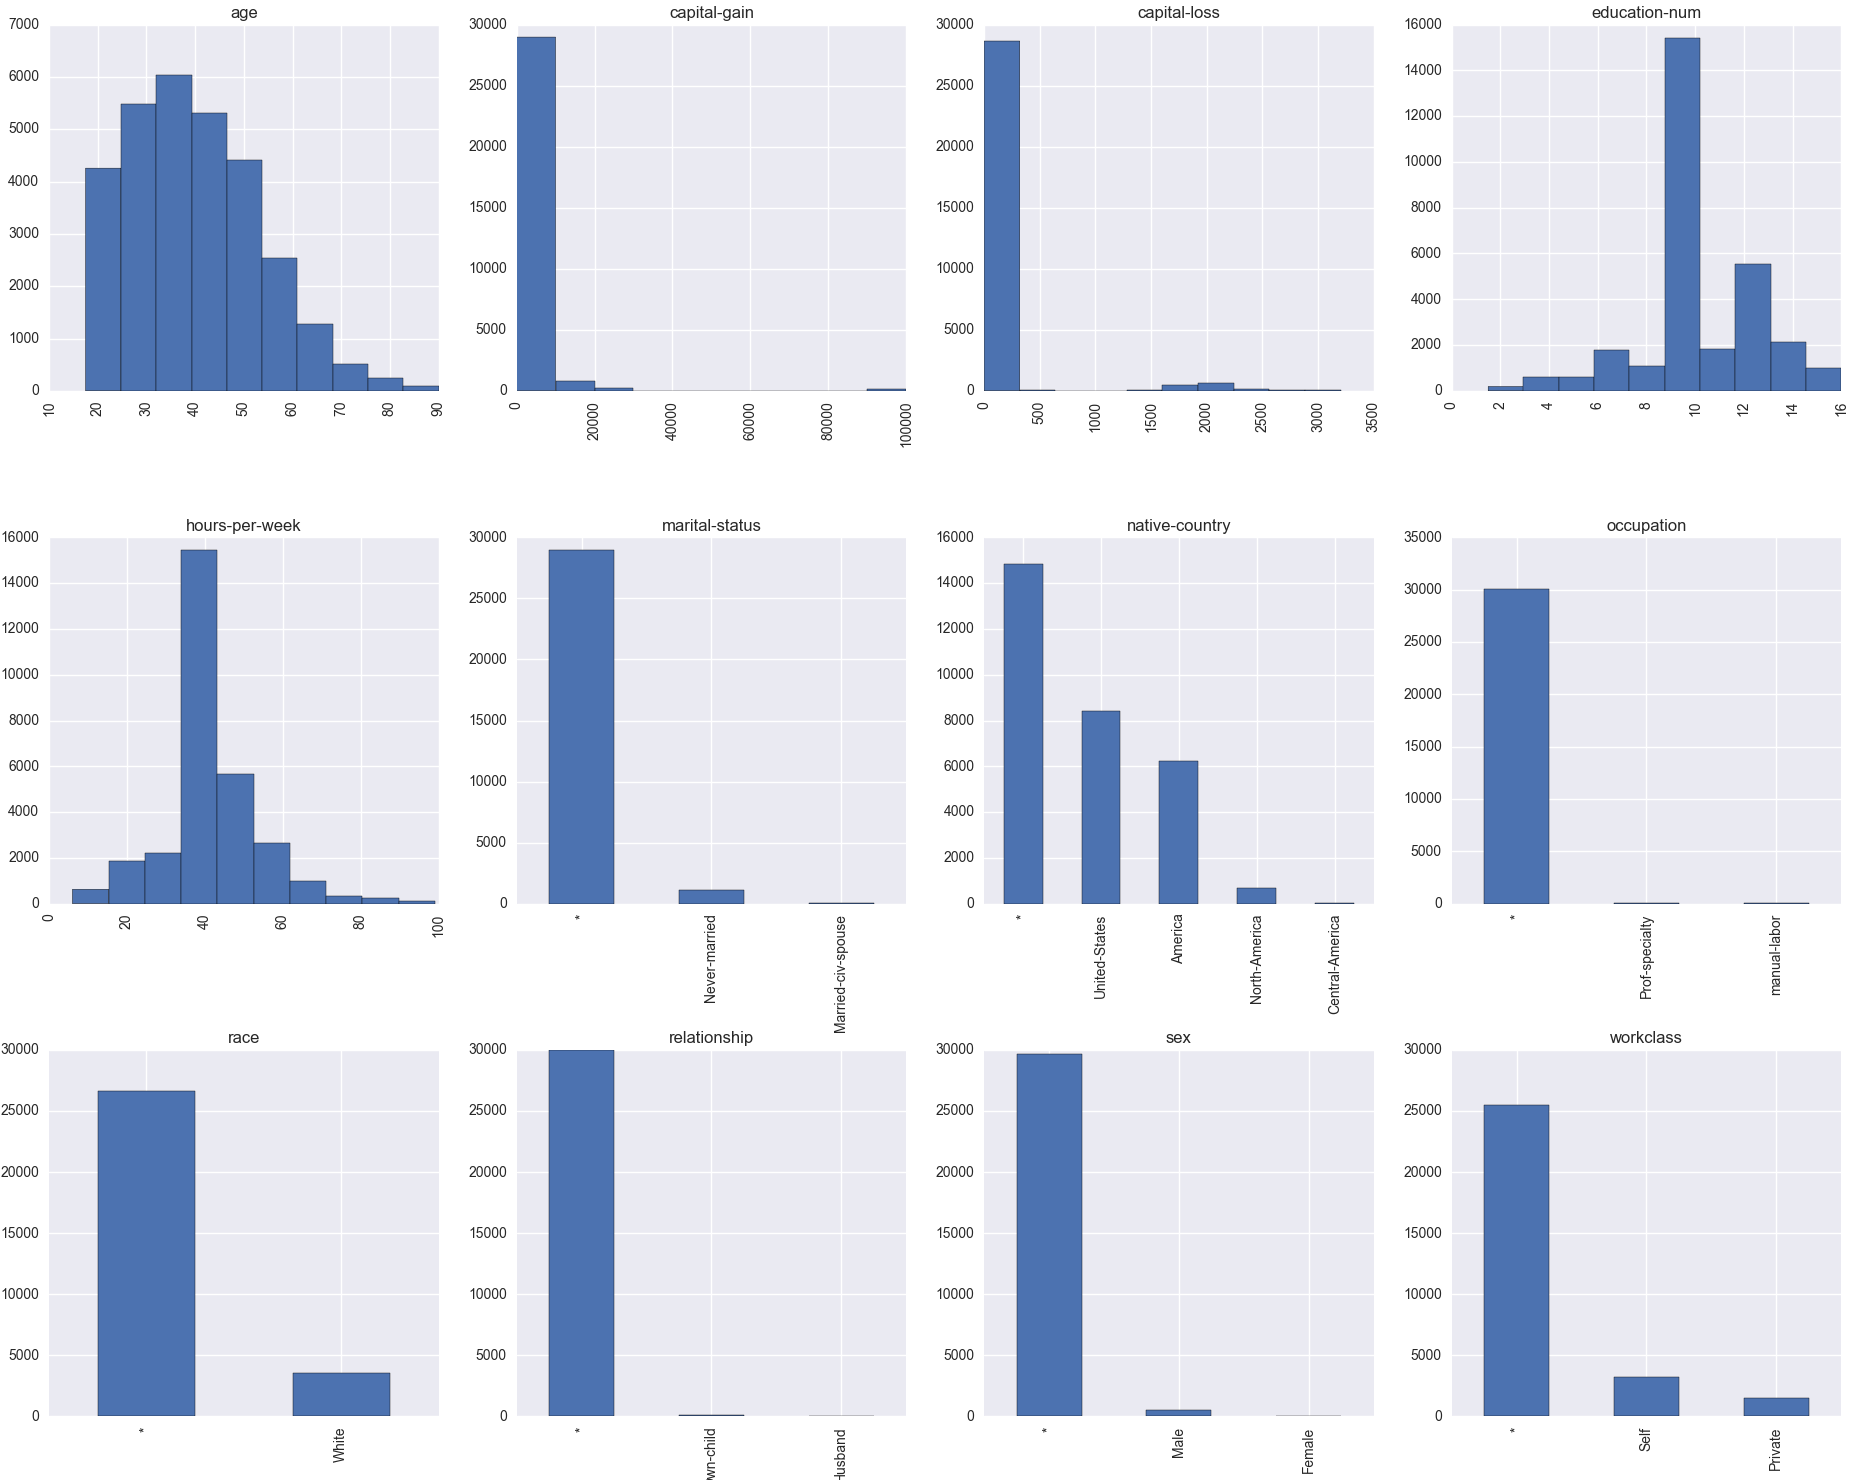
\includegraphics[width=1.2\textwidth]{figures/experiment/anon_distribution}
		\caption{Distribution of the data columns of the adult dataset with an anonymization factor of k=19}
		\label{fig:adult_anonymized_distribution}
	\end{center}
\end{figure}


\subsection{Process}
\label{ssect:process}

\begin{figure}[H]
	\begin{center}
    	\hspace*{-1.5cm}
		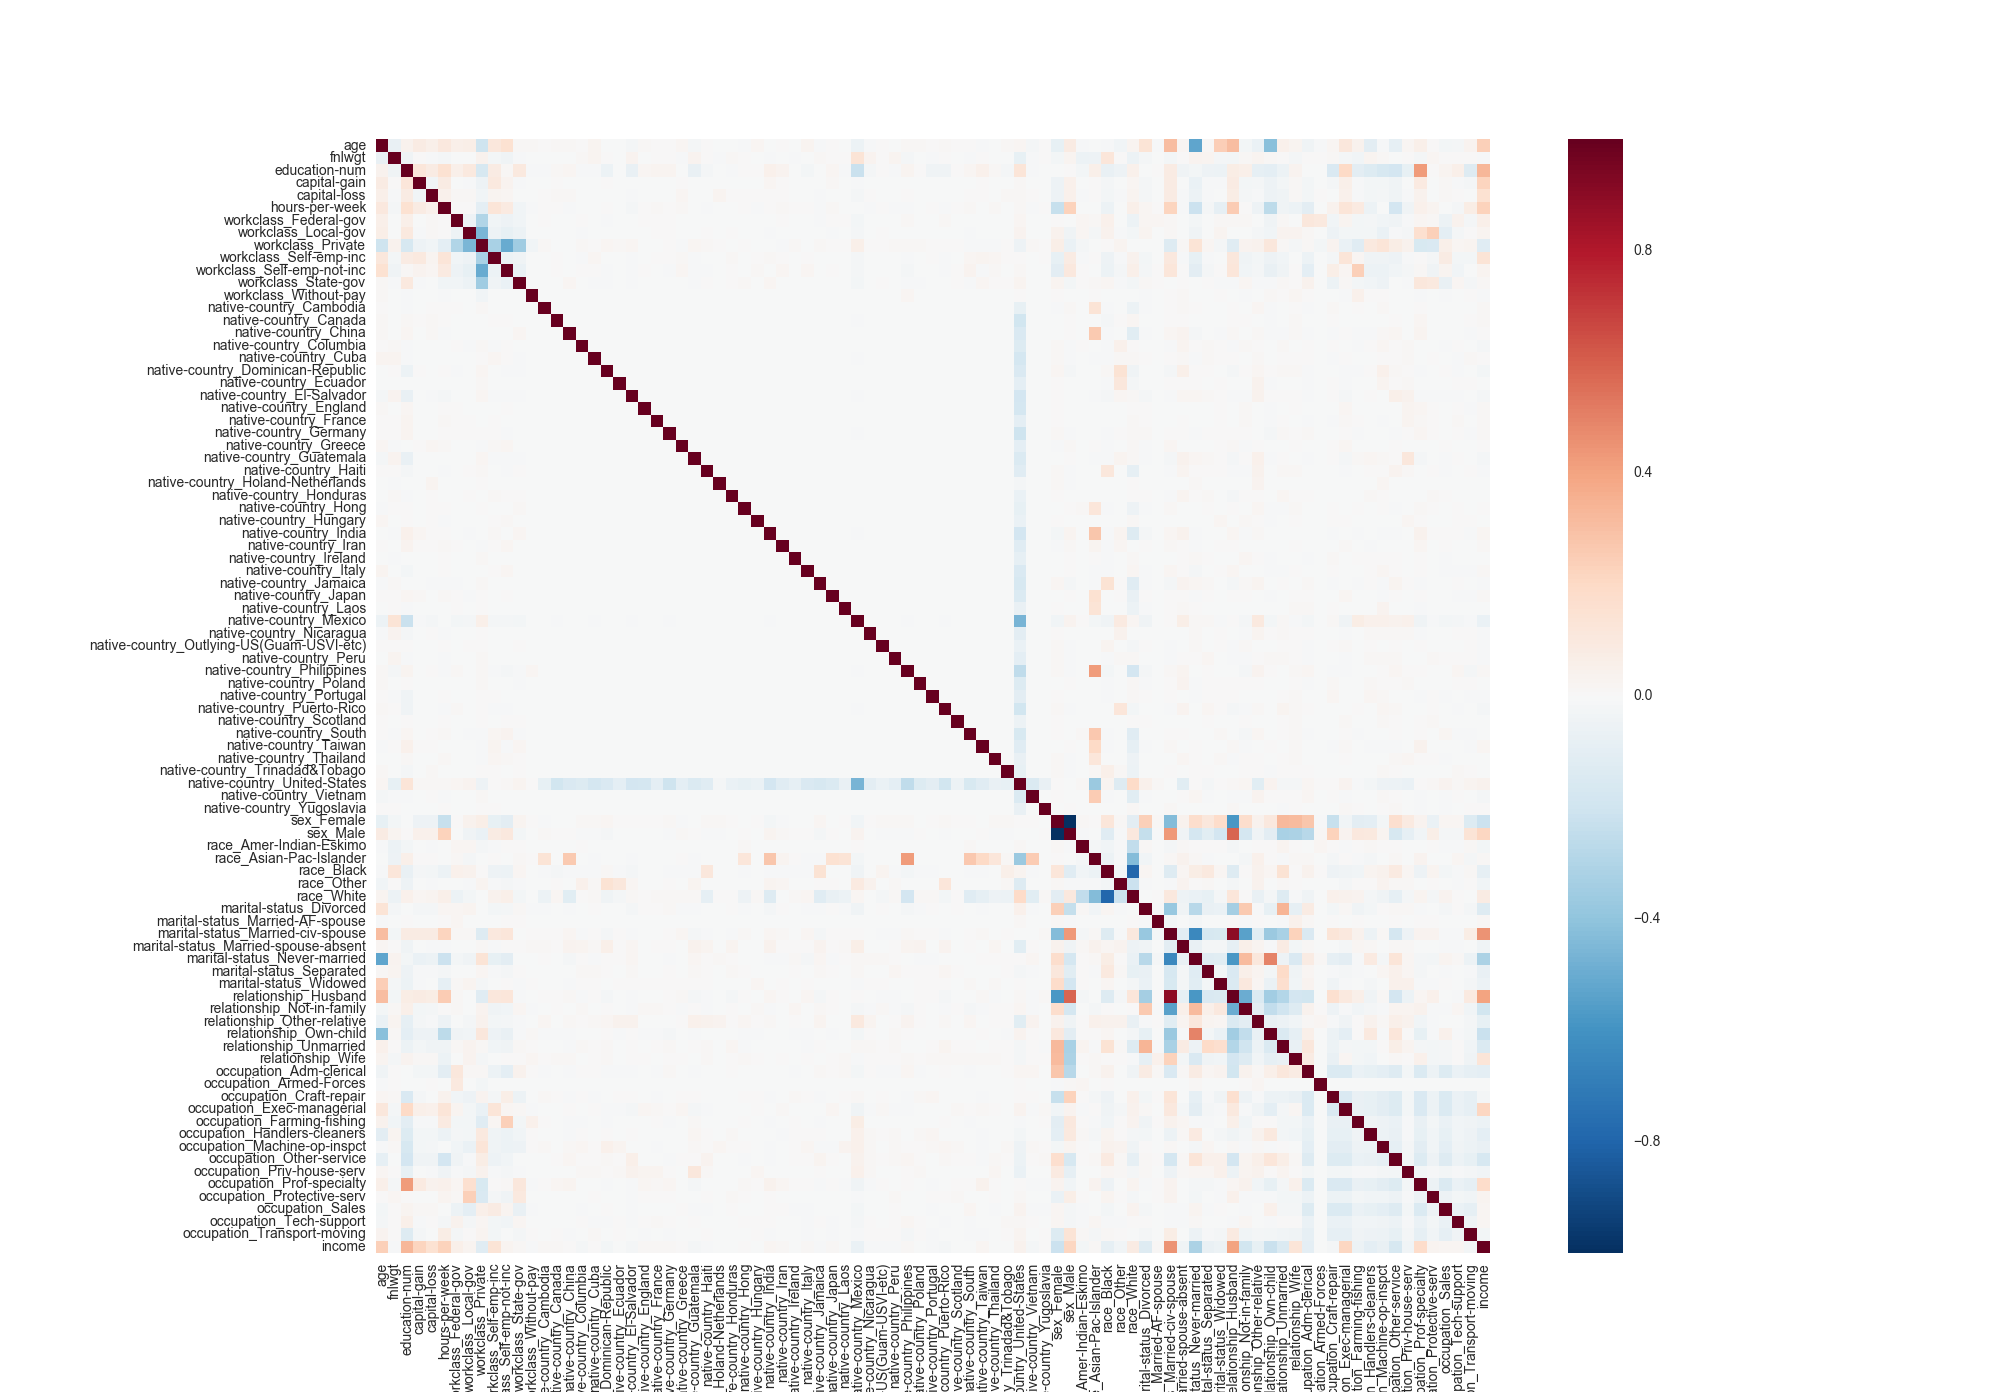
\includegraphics[width=1.3\textwidth]{figures/experiment/correlation_big}
		\caption{Correlation matrix of the attribute values of the adult dataset}
		\label{fig:adult_correlation_big}
	\end{center}
\end{figure}

\begin{figure}[H]
	\begin{center}
    	\hspace*{-1.5cm}
		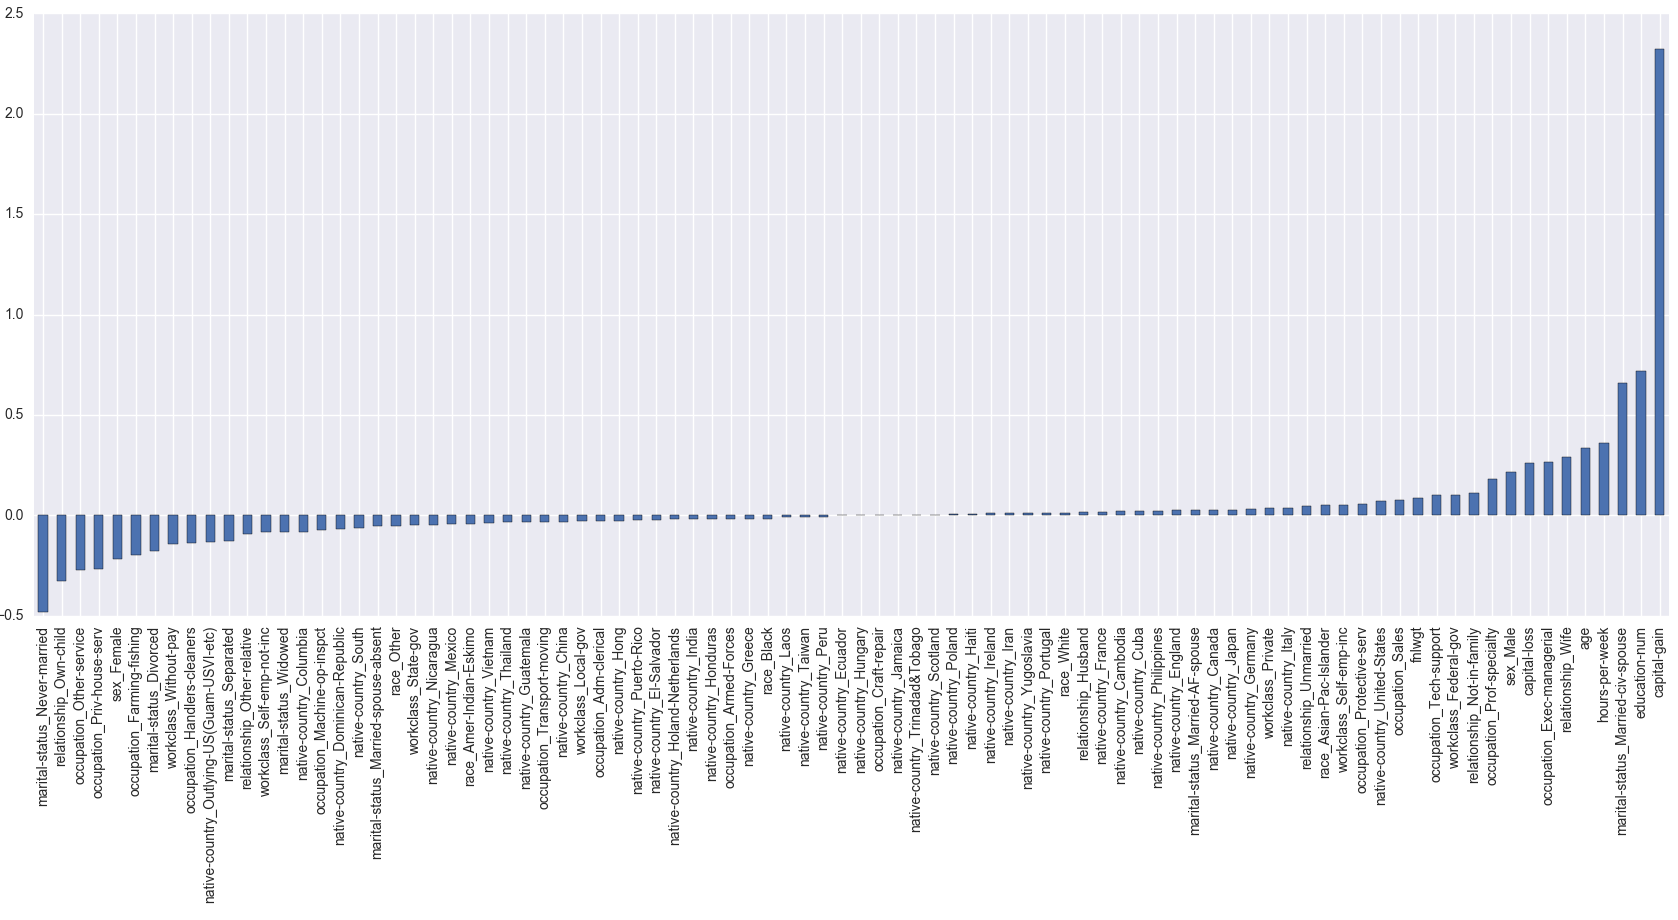
\includegraphics[width=1.3\textwidth]{figures/experiment/important_columns}
		\caption{The attribute values of the adult dataset which contribute most positively / negatively to the classification result}
		\label{fig:adult_important_columns}
	\end{center}
\end{figure}


\subsection{Algorithm}
\label{ssect:algorithm}

SaNGreeA stands for \textit{Social network greedy clustering} and was introduced by \cite{campan2009data}. In addition to 'clustering' nodes of a graph according to the minimum general information loss (GIL) incurred as described in Section~\ref{sect:graph_sn_anon}, this algorithm also considers the structural information loss (SIL) by assigning a node to a certain cluster. The SIL quantifies the probability of error when trying to reconstruct the structure of the initial graph from its anonymized version.

The SIL is composed of two different components: 1) the intra-cluster structural loss, signifying the error probability in trying to reconstruct the original edge distribution within an equivalence class (= anonymized cluster), and 2) the inter-cluster structural loss which represents the error probability in trying to reconstruct the original configuration of edges between two equivalence classes.

In implementing and demonstrating this algorithm, I recreated the paper's original experiment:

\begin{enumerate}
	\item \textbf{Process input data into suitable structure.} The adults dataset was selected and all but six columns deleted - only Age, Workclass, Country of origin, Gender, Race and Marital status remained (a sample containing the first 19 rows can be seen in Figure~\ref{fig:adult_input_data_sample}). Furthermore, in order to obtain repeatable results, the first 300 'pure' rows (no missing or mis-formatted values) in the dataset were chosen as input set.
	
	\item \textbf{Enhance structure with graph information (random edges).} Using GraphiniusJS's capability of randomly adding edges to nodes, a connected graph was created out of the assortment of nodes (using between 1 and 10 outgoing edges per node).
	

	\item \textbf{Compute GIL \& NGIL.} The general information loss with respect to a cluster is given by the following formula (repeating from the original paper):
	\begin{equation*}
    \begin{split}
	\text{GIL}(cl) = \abs{cl} \cdot (\sum_{j=1}^{s} \frac{size(gen(cl)[N_j])}{size(min_{x \epsilon N} (X[N_j]), max_{x \epsilon N} (X[N_j]))} \\ 
    + \sum_{j=1}^{t} \frac{height(\Lambda(gen(cl)[C_j]))}{height(H_{C_j})})    
    \end{split}    
	\end{equation*}
    
    
	where:\\
	- $\abs{cl}$ denotes the cluster cl's cardinality; \\
	- $size([i1,i2])$ is the size of the interval $[i1,i2]$, i.e., $(i2-i1)$; \\
	- $\Lambda(w), w \epsilon H_{C_j}$ is the subhierarchy of $H_{C_j}$ rooted in $w$; \\
	- $height(H_{C_j})$ denotes the height of the tree hierarchy $H_{C_j}$; \\
	
	The total generalization information loss is then given by:
	\begin{equation*}
	\text{GIL}(G,S) = \sum_{j=1}^{v} \text{GIL}(cl_j)
	\end{equation*}
	And the normalized generalization information loss by:
	\begin{equation*}
	\text{NGIL}(G,S) = \frac{\text{GIL}(G,S)}{n \cdot (s+t)}
	\end{equation*}
	
	\item \textbf{Compute SIL \& NSIL.} For the exact mathematical definitions of SIL \& NSIL the reader is kindly referred to the original paper. Because the structural information loss cannot be computed exactly before the final construction of clusters, the exact computations were replaced by the following distance measures: \\
	Distance between two nodes:
	\begin{equation*}
	\text{dist}(X^i, X^j) = \frac{\abs{\{l|l=1..n \wedge l \ne i,j;b_l^i \ne b_l^j}}{n-2}
	\end{equation*}
	
	Distance between a node and a cluster:
	\begin{equation*}
	\text{dist}(X, cl) = \frac{\sum_{X^j \epsilon cl} \text{dist}(X, X^j) }{\abs{cl}}
	\end{equation*}
\end{enumerate}

The algorithm starts with initializing a first cluster by simply adding a randomly chosen node to it. Then, for every new node encountered, the weighted sum of the above two information loss metrics will yield a certain overall information loss value if the node was added to that cluster - the node with the minimal cost is then chosen as the candidate and expands the cluster. This is repeated until the first cluster reaches a certain requirement (e.g. size $ \coloneqq  k $ -factor) upon which another random node is chosen to constitute a next cluster. This procedure is repeated until all nodes have been assigned (if a cluster of size < k-factor remains, its member nodes are dispersed amongst the others). 

Since the algorithm does not take ALL possible node combinations into account, but simply start with a node and compares all the candidates in a loop, the algorithm runs in quadratic time w.r.t. the input size in number of nodes. This worked well within milliseconds for an input problem size of a few hundred nodes. An example output of the implemented algorithm can be found at \hl{Enter Graphinius URL here}. \\


\section{Results}
\label{sect:results}

\begin{figure}[H]
	\begin{center}
		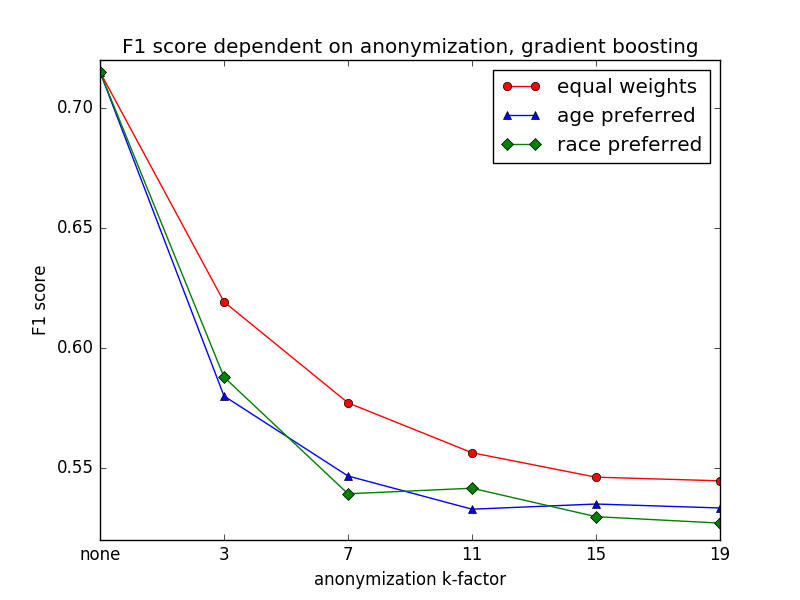
\includegraphics[width=0.32\textwidth]{figures/results/anon_gradient_boost}
		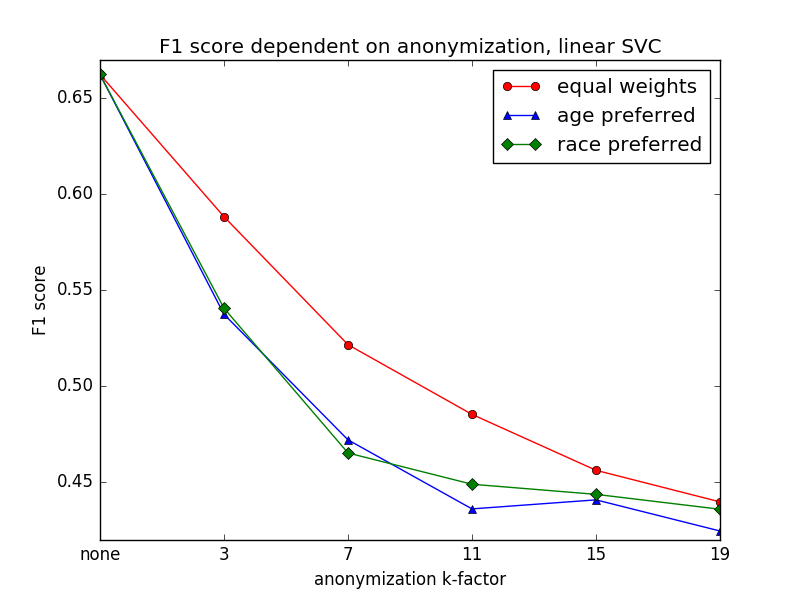
\includegraphics[width=0.32\textwidth]{figures/results/anon_linear_svc}
		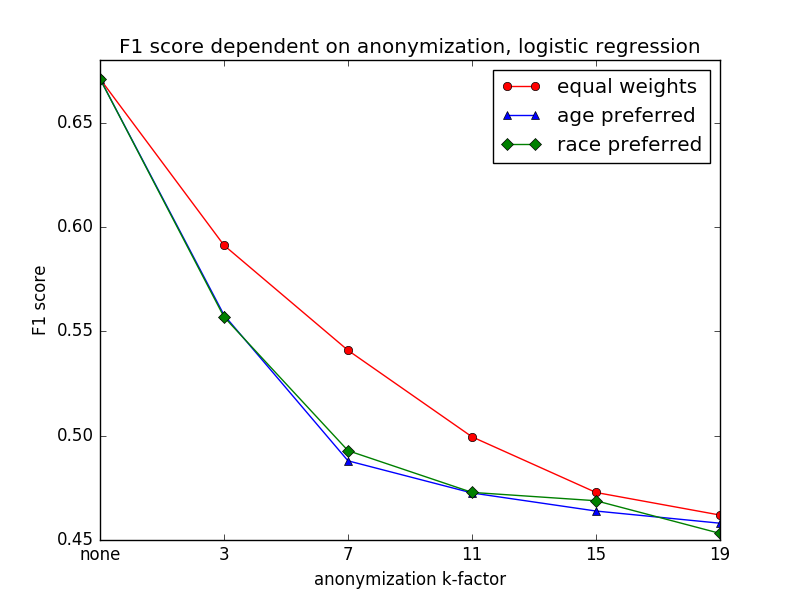
\includegraphics[width=0.32\textwidth]{figures/results/anon_logistic_regression}
		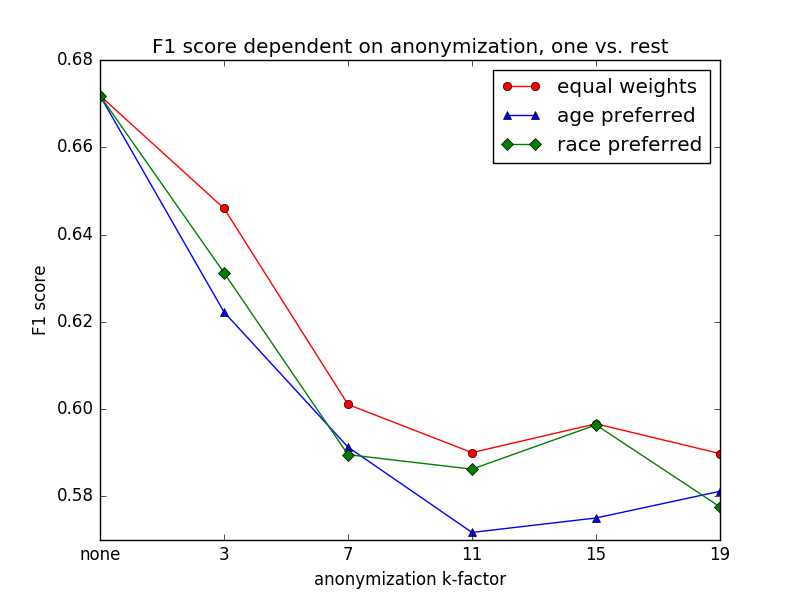
\includegraphics[width=0.32\textwidth]{figures/results/anon_onevsrest_bagging}
		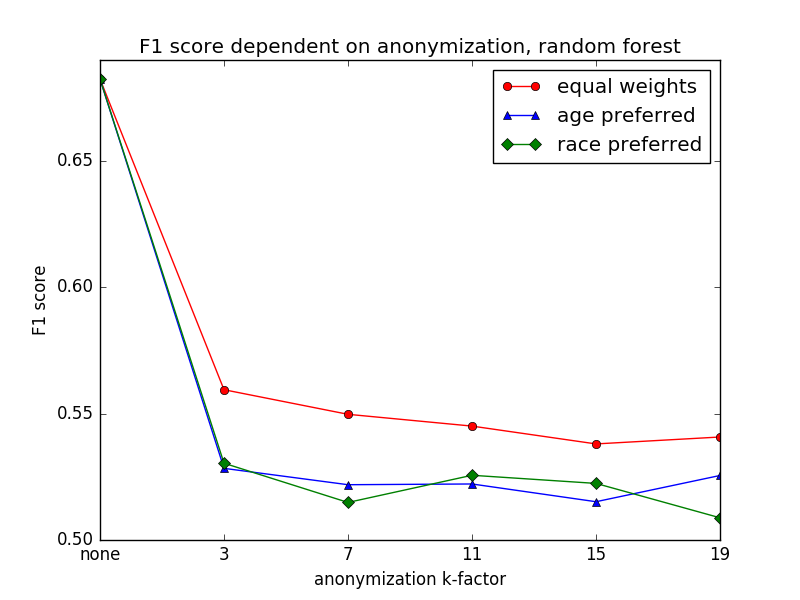
\includegraphics[width=0.32\textwidth]{figures/results/anon_random_forest}
		\caption{The impact of anonymization on the F1 score of different classifiers}
		\label{fig:adult_results_anonymization}
	\end{center}
\end{figure}

\begin{figure}[H]
	\begin{center}
		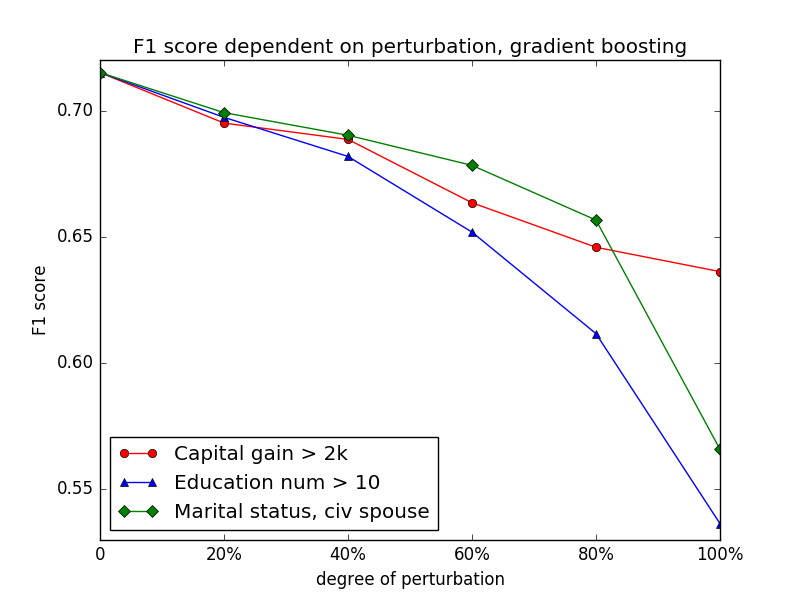
\includegraphics[width=0.32\textwidth]{figures/results/perturb_gradient_boost}
		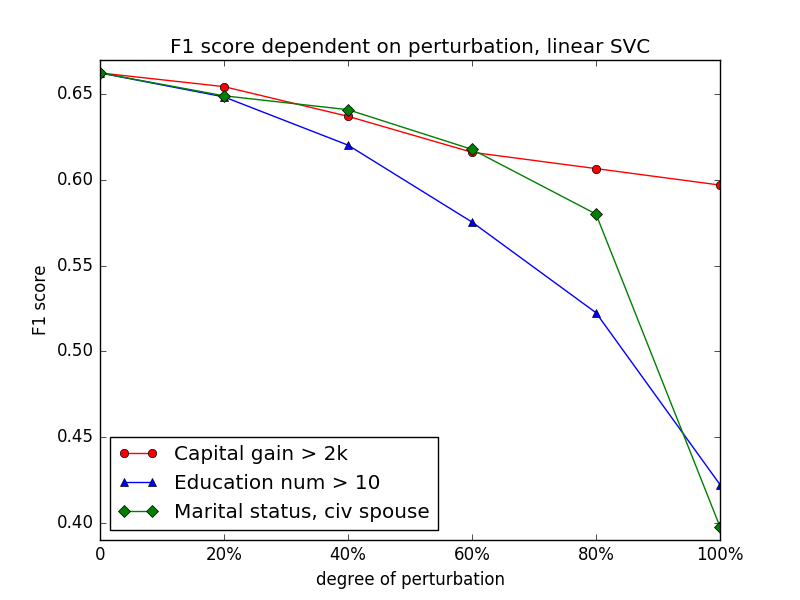
\includegraphics[width=0.32\textwidth]{figures/results/perturb_linear_svc}
		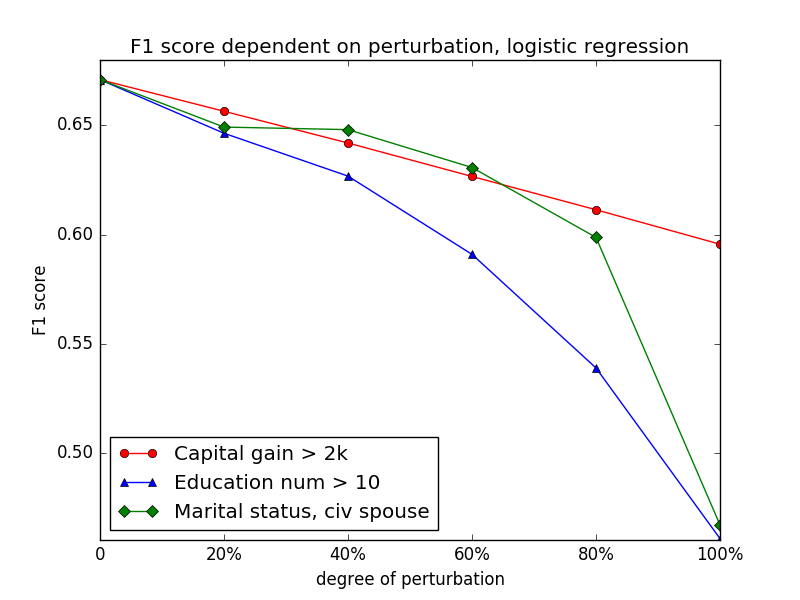
\includegraphics[width=0.32\textwidth]{figures/results/perturb_logistic_regression}
		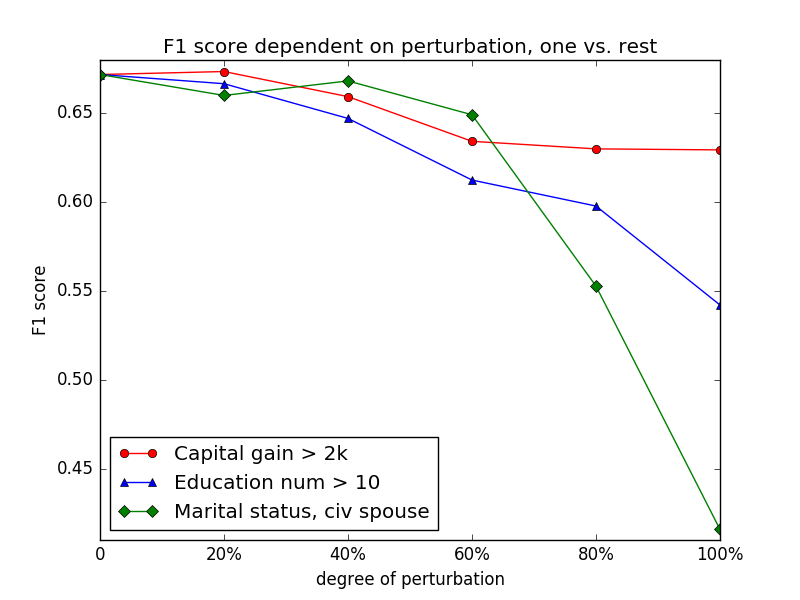
\includegraphics[width=0.32\textwidth]{figures/results/perturb_onevsrest_bagging}
		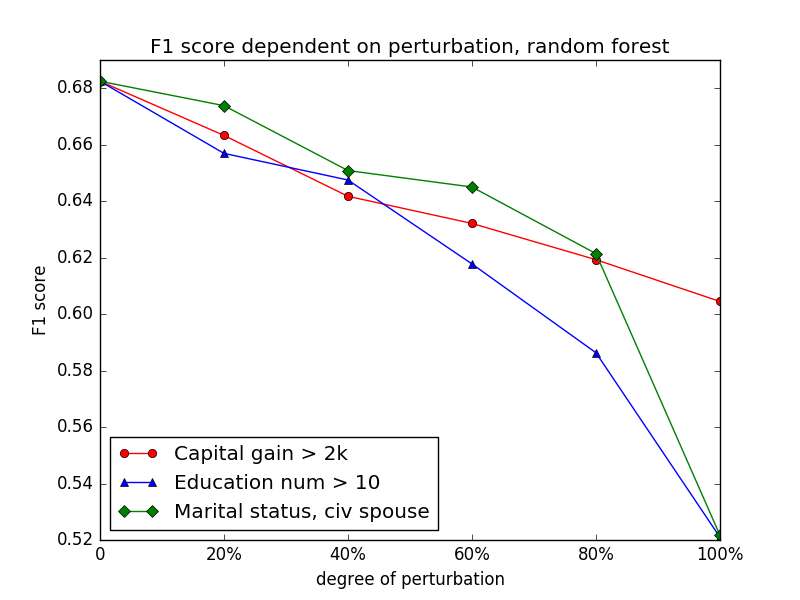
\includegraphics[width=0.32\textwidth]{figures/results/perturb_random_forest}
		\caption{The impact of perturbation (selectively deleting quantiles of rows containing one of the TOP 3 contributing attributes) on the F1 score of different classifiers}
		\label{fig:adult_results_perturbation_top}
	\end{center}
\end{figure}

\begin{figure}[H]
	\begin{center}
		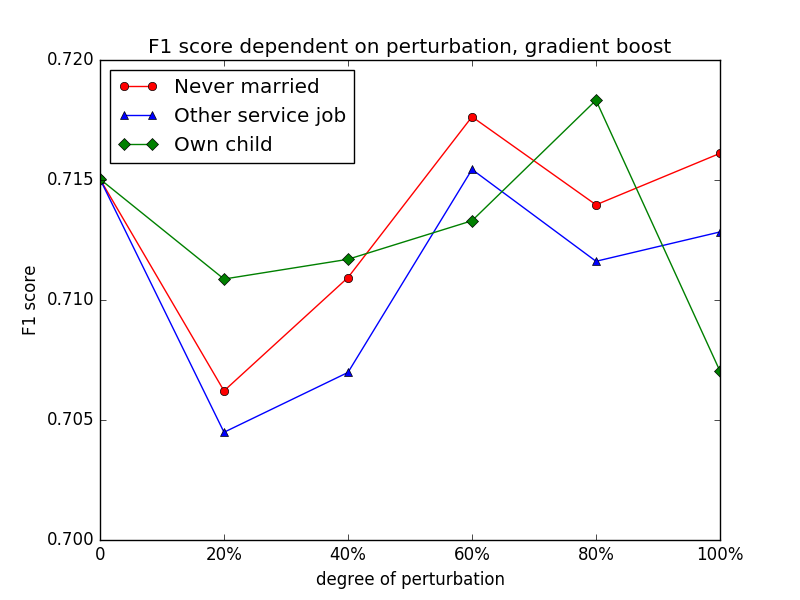
\includegraphics[width=0.32\textwidth]{figures/results/perturb_gradient_boost_bottom}
		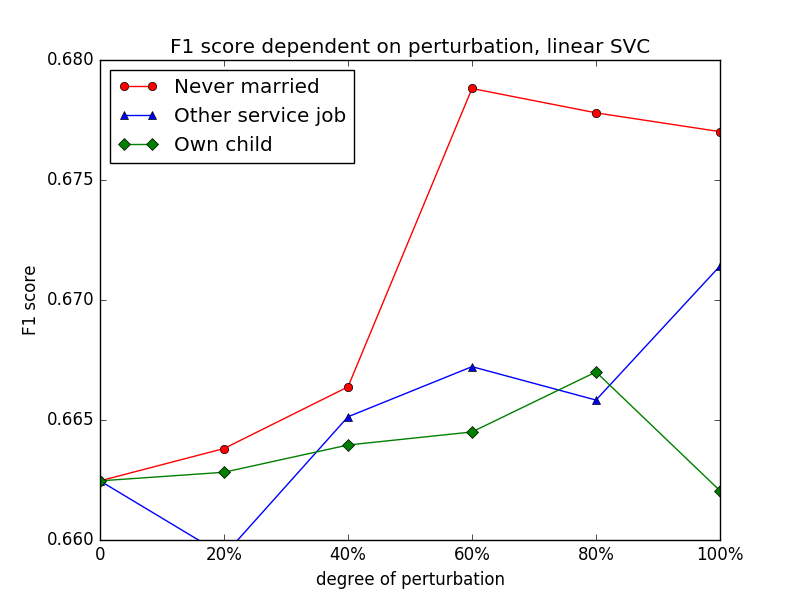
\includegraphics[width=0.32\textwidth]{figures/results/perturb_linear_svc_bottom}
		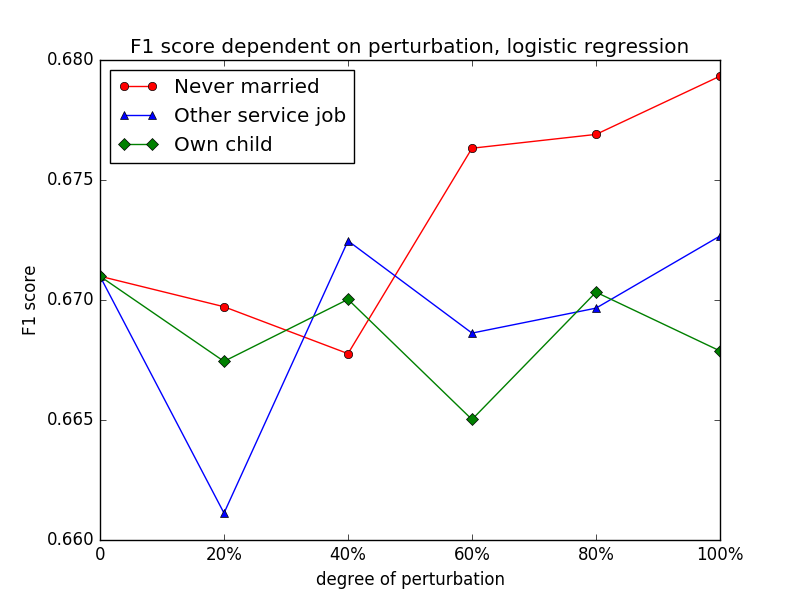
\includegraphics[width=0.32\textwidth]{figures/results/perturb_logistic_regression_bottom}
		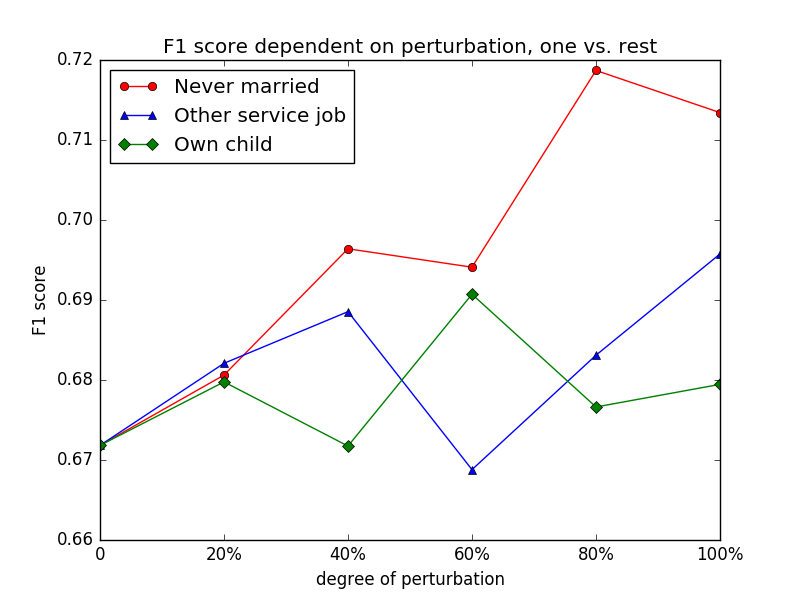
\includegraphics[width=0.32\textwidth]{figures/results/perturb_onevsrest_bagging_bottom}
		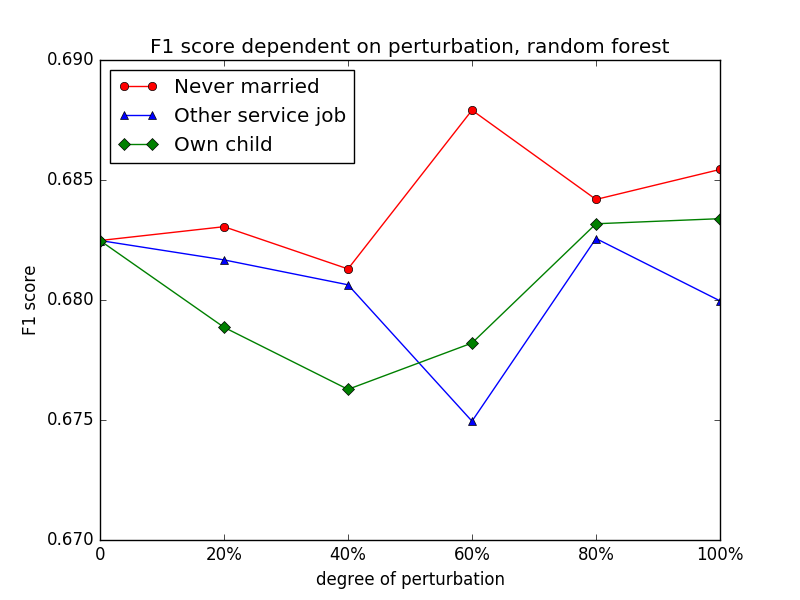
\includegraphics[width=0.32\textwidth]{figures/results/perturb_random_forest_bottom}
		\caption{The impact of perturbation (selectively deleting quantiles of rows containing one of the BOTTOM 3 contributing attributes) on the F1 score of different classifiers}
		\label{fig:adult_results_perturbation_top}
	\end{center}
\end{figure}



\section{Discussion}
\label{sect:discussion}


\section{Open problems and future challenges}
\label{sect:op_fc}


\section{Conclusion}
\label{sect:conclusion}



\newpage

\bibliographystyle{plain}
\bibliography{references}

\end{document}
